\documentclass{article}
\usepackage[utf8]{inputenc}
\usepackage{graphicx}

\title{Reporte 1: Busqueda Lineal\\\textbf{Análisis de Algoritmos}}
\author{ Ramiro Estrada García\\2015190034 }
\date{15 de Octubre del 2020}

\begin{document}
\maketitle
\vspace{5cm}
\section {Características del PC}
\begin{itemize}
	\item CPU: Intel Core i5 9700F a 4.1GHz
	\item RAM: 16GB a 2666MHz
\end{itemize}
\newpage
\maketitle
\section{Mejor caso}
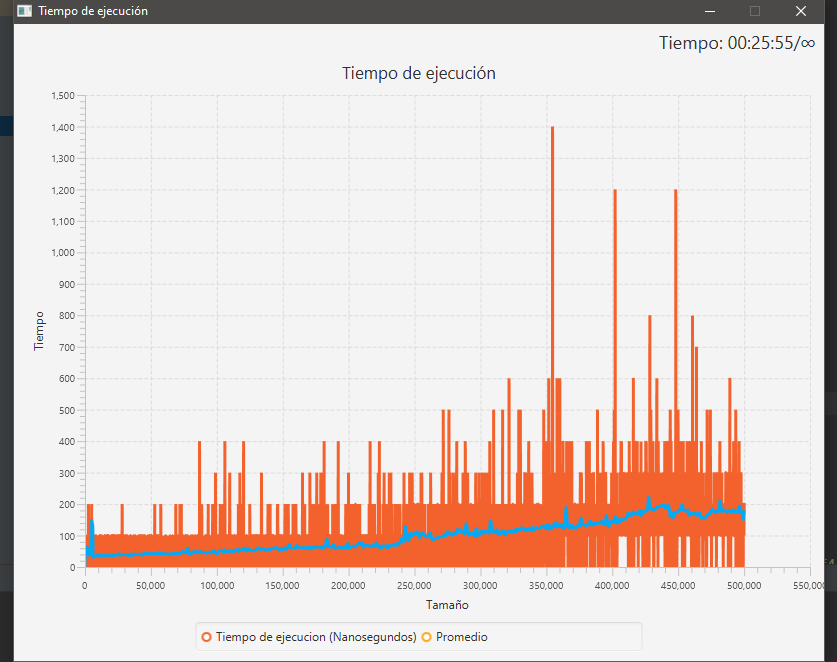
\includegraphics[width=12cm]{mejor.png}\\
En este caso, los datos siempre van a tener el elemento a buscar en la primer posición. 
Es por esto que en las iteraciones tienen un rango de $[0,1400]$ nanosegundos y en promedio entre $[30, 230]$ nanosegundos.
\maketitle
\section{Medio caso}
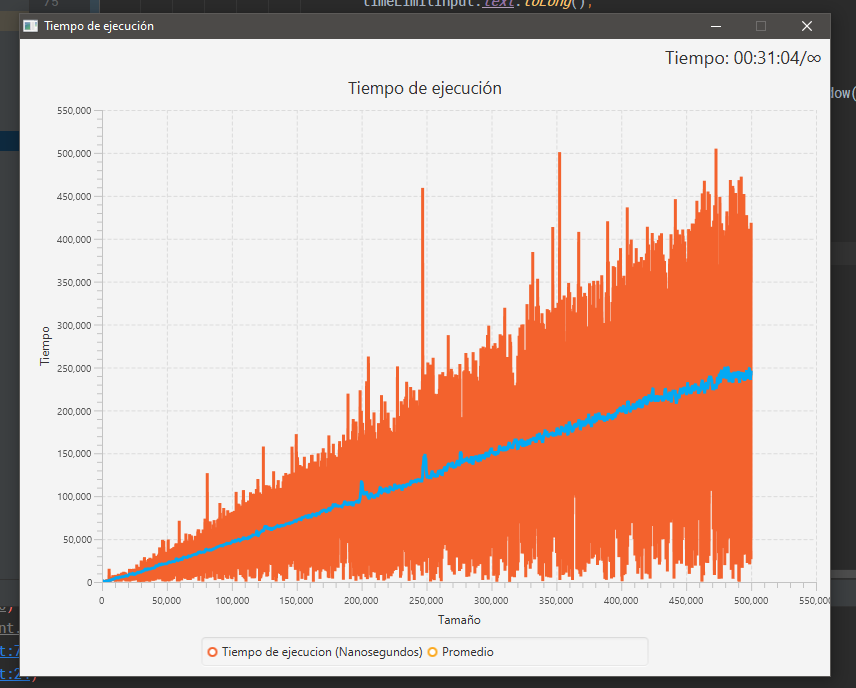
\includegraphics[width=12cm]{medio.png}\\
En este caso, el dato a buscar está en cualquier posición del arreglo por lo que puede estar en la primer posición o puede estar en la última posición. 
En la gráfica, se hace notar el hecho anterior al cubrir toda el area desde el mejor caso hasta el peor caso. Los datos van desde $[0,500000]$ nanosegundos y en promedio entre $[0,250000]$.
\maketitle
\section{Peor caso}
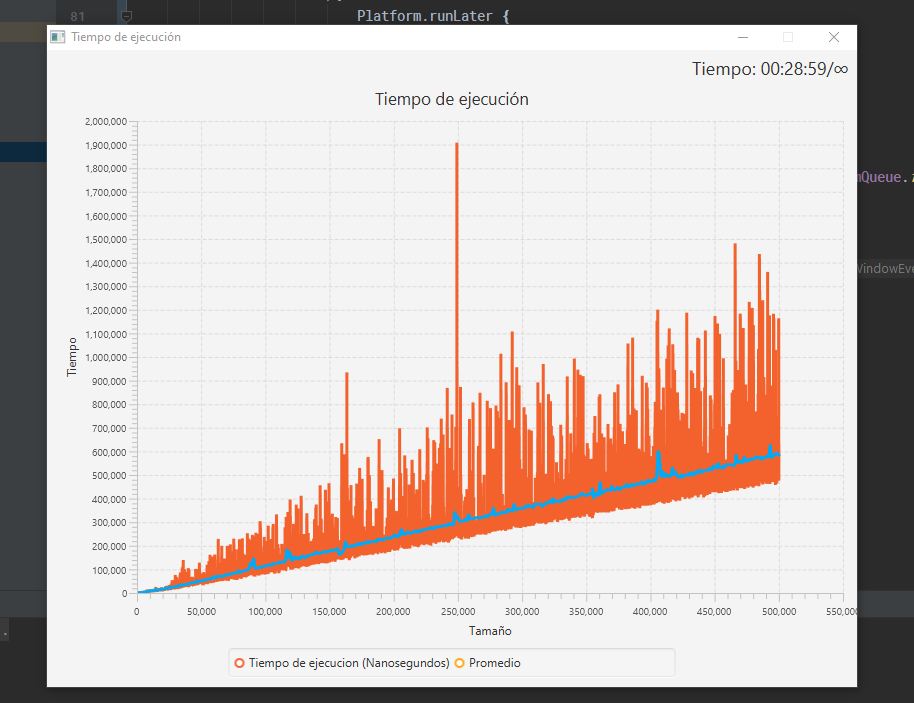
\includegraphics[width=12cm]{peor.png}\\
En este caso, el arreglo siempre va a tener los datos en el último elemento por lo que el algoritmo tiene que analizar hasta el final para encontrar el valor. 
En la gráfica se nota la ausencia de datos en la parte inferior por la razón anterior. Los datos van de $[0, 1900000]$ nanosegundos con un promedio de $[0, 550000]$ nanosegundos.
\end{document}